% Created by tikzDevice version 0.12.3 on 2020-10-30 19:57:42
% !TEX encoding = UTF-8 Unicode
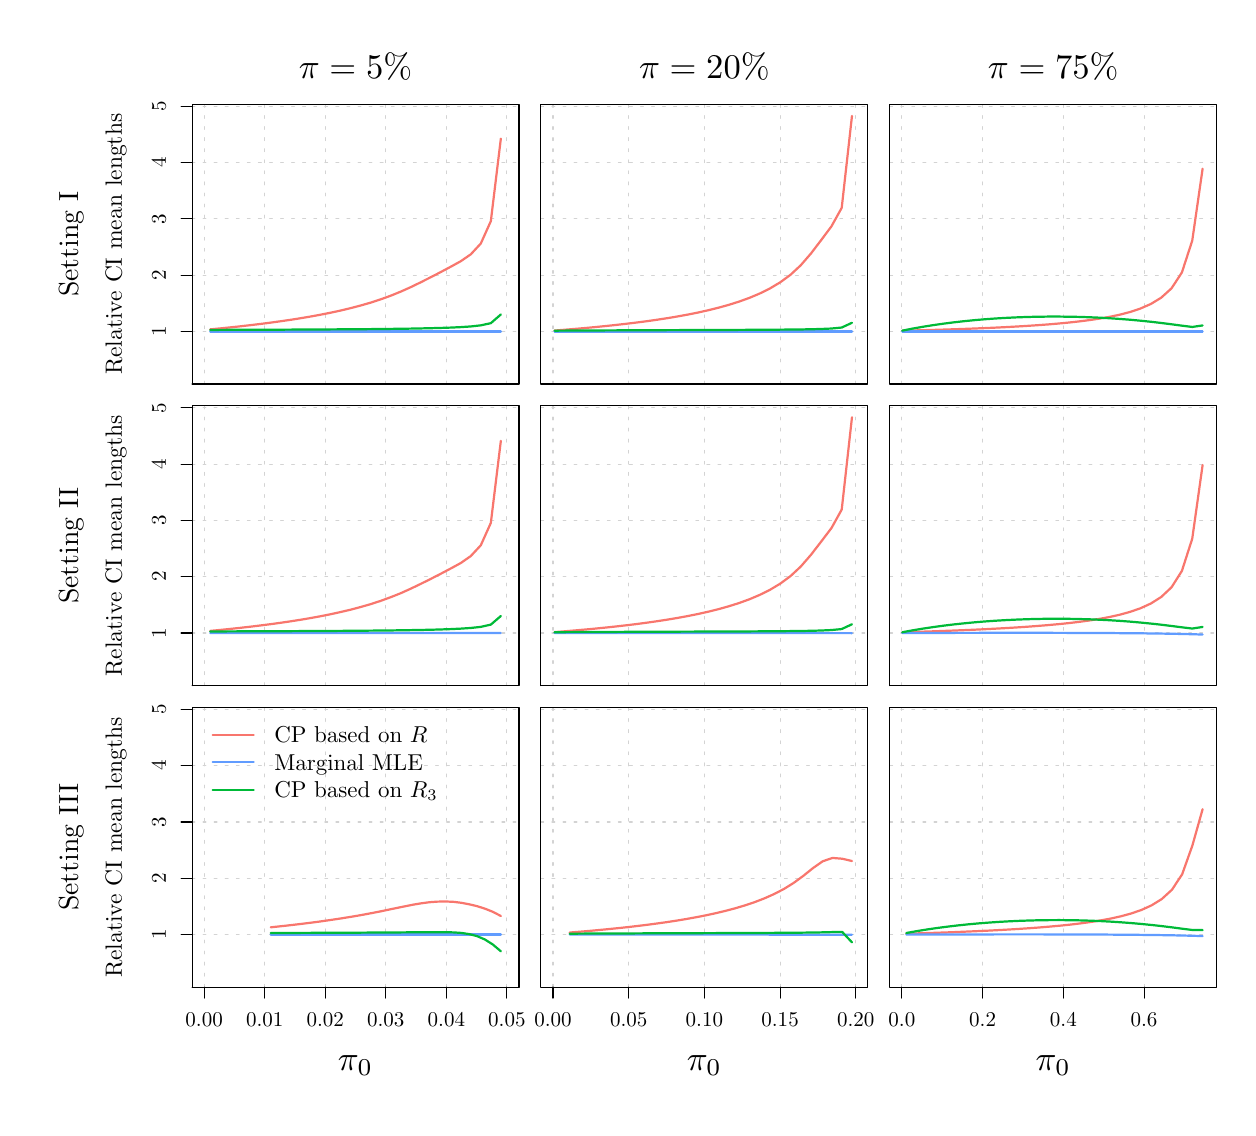
\begin{tikzpicture}[x=1pt,y=1pt]
\definecolor{fillColor}{RGB}{255,255,255}
\path[use as bounding box,fill=fillColor,fill opacity=0.00] (0,0) rectangle (433.62,390.26);
\begin{scope}
\path[clip] ( 55.44,257.53) rectangle (181.50,366.50);
\definecolor{drawColor}{RGB}{0,0,0}

\node[text=drawColor,anchor=base,inner sep=0pt, outer sep=0pt, scale=  0.66] at (118.47,231.40) {Simulation ID};

\node[text=drawColor,rotate= 90.00,anchor=base,inner sep=0pt, outer sep=0pt, scale=  0.66] at ( 34.06,312.01) {Ratio of RMSE};
\end{scope}
\begin{scope}
\path[clip] (  0.00,  0.00) rectangle (433.62,390.26);
\definecolor{drawColor}{RGB}{0,0,0}

\path[draw=drawColor,line width= 0.4pt,line join=round,line cap=round] ( 59.40,280.49) -- ( 59.40,361.85);

\path[draw=drawColor,line width= 0.4pt,line join=round,line cap=round] ( 59.40,280.49) -- ( 55.44,280.49);

\path[draw=drawColor,line width= 0.4pt,line join=round,line cap=round] ( 59.40,300.83) -- ( 55.44,300.83);

\path[draw=drawColor,line width= 0.4pt,line join=round,line cap=round] ( 59.40,321.17) -- ( 55.44,321.17);

\path[draw=drawColor,line width= 0.4pt,line join=round,line cap=round] ( 59.40,341.51) -- ( 55.44,341.51);

\path[draw=drawColor,line width= 0.4pt,line join=round,line cap=round] ( 59.40,361.85) -- ( 55.44,361.85);

\node[text=drawColor,rotate= 90.00,anchor=base,inner sep=0pt, outer sep=0pt, scale=  0.76] at ( 49.90,280.49) {1};

\node[text=drawColor,rotate= 90.00,anchor=base,inner sep=0pt, outer sep=0pt, scale=  0.76] at ( 49.90,300.83) {2};

\node[text=drawColor,rotate= 90.00,anchor=base,inner sep=0pt, outer sep=0pt, scale=  0.76] at ( 49.90,321.17) {3};

\node[text=drawColor,rotate= 90.00,anchor=base,inner sep=0pt, outer sep=0pt, scale=  0.76] at ( 49.90,341.51) {4};

\node[text=drawColor,rotate= 90.00,anchor=base,inner sep=0pt, outer sep=0pt, scale=  0.76] at ( 49.90,361.85) {5};
\end{scope}
\begin{scope}
\path[clip] ( 59.40,261.49) rectangle (177.54,362.54);
\definecolor{drawColor}{RGB}{211,211,211}

\path[draw=drawColor,line width= 0.4pt,dash pattern=on 1pt off 3pt ,line join=round,line cap=round] ( 63.78,261.49) -- ( 63.78,362.54);

\path[draw=drawColor,line width= 0.4pt,dash pattern=on 1pt off 3pt ,line join=round,line cap=round] ( 85.65,261.49) -- ( 85.65,362.54);

\path[draw=drawColor,line width= 0.4pt,dash pattern=on 1pt off 3pt ,line join=round,line cap=round] (107.53,261.49) -- (107.53,362.54);

\path[draw=drawColor,line width= 0.4pt,dash pattern=on 1pt off 3pt ,line join=round,line cap=round] (129.41,261.49) -- (129.41,362.54);

\path[draw=drawColor,line width= 0.4pt,dash pattern=on 1pt off 3pt ,line join=round,line cap=round] (151.29,261.49) -- (151.29,362.54);

\path[draw=drawColor,line width= 0.4pt,dash pattern=on 1pt off 3pt ,line join=round,line cap=round] (173.16,261.49) -- (173.16,362.54);

\path[draw=drawColor,line width= 0.4pt,dash pattern=on 1pt off 3pt ,line join=round,line cap=round] ( 59.40,280.49) -- (177.54,280.49);

\path[draw=drawColor,line width= 0.4pt,dash pattern=on 1pt off 3pt ,line join=round,line cap=round] ( 59.40,300.83) -- (177.54,300.83);

\path[draw=drawColor,line width= 0.4pt,dash pattern=on 1pt off 3pt ,line join=round,line cap=round] ( 59.40,321.17) -- (177.54,321.17);

\path[draw=drawColor,line width= 0.4pt,dash pattern=on 1pt off 3pt ,line join=round,line cap=round] ( 59.40,341.51) -- (177.54,341.51);

\path[draw=drawColor,line width= 0.4pt,dash pattern=on 1pt off 3pt ,line join=round,line cap=round] ( 59.40,361.85) -- (177.54,361.85);
\end{scope}
\begin{scope}
\path[clip] (  0.00,  0.00) rectangle (433.62,390.26);
\definecolor{drawColor}{RGB}{0,0,0}

\path[draw=drawColor,line width= 0.4pt,line join=round,line cap=round] ( 59.40,261.49) --
	(177.54,261.49) --
	(177.54,362.54) --
	( 59.40,362.54) --
	( 59.40,261.49);
\end{scope}
\begin{scope}
\path[clip] ( 59.40,261.49) rectangle (177.54,362.54);
\definecolor{drawColor}{RGB}{248,118,109}

\path[draw=drawColor,line width= 0.8pt,line join=round,line cap=round] ( 65.96,281.24) --
	( 69.58,281.59) --
	( 73.21,281.96) --
	( 76.83,282.34) --
	( 80.45,282.76) --
	( 84.07,283.19) --
	( 87.69,283.66) --
	( 91.31,284.16) --
	( 94.93,284.68) --
	( 98.55,285.25) --
	(102.17,285.87) --
	(105.80,286.53) --
	(109.42,287.25) --
	(113.04,288.03) --
	(116.66,288.90) --
	(120.28,289.85) --
	(123.90,290.89) --
	(127.52,292.07) --
	(131.14,293.39) --
	(134.77,294.86) --
	(138.39,296.48) --
	(142.01,298.24) --
	(145.63,300.07) --
	(149.25,301.94) --
	(152.87,303.87) --
	(156.49,305.86) --
	(160.11,308.35) --
	(163.73,312.25) --
	(167.36,320.33) --
	(170.98,350.17);
\definecolor{drawColor}{RGB}{97,156,255}

\path[draw=drawColor,line width= 0.8pt,line join=round,line cap=round] ( 65.96,280.49) --
	( 69.58,280.49) --
	( 73.21,280.49) --
	( 76.83,280.49) --
	( 80.45,280.49) --
	( 84.07,280.49) --
	( 87.69,280.49) --
	( 91.31,280.49) --
	( 94.93,280.49) --
	( 98.55,280.49) --
	(102.17,280.49) --
	(105.80,280.49) --
	(109.42,280.49) --
	(113.04,280.49) --
	(116.66,280.49) --
	(120.28,280.49) --
	(123.90,280.49) --
	(127.52,280.49) --
	(131.14,280.49) --
	(134.77,280.49) --
	(138.39,280.49) --
	(142.01,280.49) --
	(145.63,280.49) --
	(149.25,280.49) --
	(152.87,280.49) --
	(156.49,280.49) --
	(160.11,280.49) --
	(163.73,280.49) --
	(167.36,280.49) --
	(170.98,280.49);
\definecolor{drawColor}{RGB}{0,186,56}

\path[draw=drawColor,line width= 0.8pt,line join=round,line cap=round] ( 65.96,281.04) --
	( 69.58,281.05) --
	( 73.21,281.07) --
	( 76.83,281.08) --
	( 80.45,281.09) --
	( 84.07,281.10) --
	( 87.69,281.12) --
	( 91.31,281.13) --
	( 94.93,281.15) --
	( 98.55,281.17) --
	(102.17,281.18) --
	(105.80,281.20) --
	(109.42,281.23) --
	(113.04,281.25) --
	(116.66,281.27) --
	(120.28,281.30) --
	(123.90,281.33) --
	(127.52,281.37) --
	(131.14,281.41) --
	(134.77,281.46) --
	(138.39,281.51) --
	(142.01,281.58) --
	(145.63,281.66) --
	(149.25,281.76) --
	(152.87,281.88) --
	(156.49,282.05) --
	(160.11,282.29) --
	(163.73,282.69) --
	(167.36,283.48) --
	(170.98,286.62);
\end{scope}
\begin{scope}
\path[clip] (  0.00,  0.00) rectangle (433.62,390.26);
\definecolor{drawColor}{RGB}{0,0,0}

\node[text=drawColor,rotate= 90.00,anchor=base,inner sep=0pt, outer sep=0pt, scale=  1.00] at ( 18.22,312.01) {Setting I};

\node[text=drawColor,rotate= 90.00,anchor=base,inner sep=0pt, outer sep=0pt, scale=  0.85] at ( 34.06,312.01) {Relative CI mean lengths};

\node[text=drawColor,anchor=base,inner sep=0pt, outer sep=0pt, scale=  1.25] at (118.47,372.04) {$\pi = 5\%$};
\end{scope}
\begin{scope}
\path[clip] (181.50,257.53) rectangle (307.56,366.50);
\definecolor{drawColor}{RGB}{0,0,0}

\node[text=drawColor,anchor=base,inner sep=0pt, outer sep=0pt, scale=  0.66] at (244.53,231.40) {Simulation ID};

\node[text=drawColor,rotate= 90.00,anchor=base,inner sep=0pt, outer sep=0pt, scale=  0.66] at (160.12,312.01) {Ratio of RMSE};
\end{scope}
\begin{scope}
\path[clip] (185.46,261.49) rectangle (303.60,362.54);
\definecolor{drawColor}{RGB}{211,211,211}

\path[draw=drawColor,line width= 0.4pt,dash pattern=on 1pt off 3pt ,line join=round,line cap=round] (189.84,261.49) -- (189.84,362.54);

\path[draw=drawColor,line width= 0.4pt,dash pattern=on 1pt off 3pt ,line join=round,line cap=round] (217.18,261.49) -- (217.18,362.54);

\path[draw=drawColor,line width= 0.4pt,dash pattern=on 1pt off 3pt ,line join=round,line cap=round] (244.53,261.49) -- (244.53,362.54);

\path[draw=drawColor,line width= 0.4pt,dash pattern=on 1pt off 3pt ,line join=round,line cap=round] (271.88,261.49) -- (271.88,362.54);

\path[draw=drawColor,line width= 0.4pt,dash pattern=on 1pt off 3pt ,line join=round,line cap=round] (299.22,261.49) -- (299.22,362.54);

\path[draw=drawColor,line width= 0.4pt,dash pattern=on 1pt off 3pt ,line join=round,line cap=round] (185.46,280.49) -- (303.60,280.49);

\path[draw=drawColor,line width= 0.4pt,dash pattern=on 1pt off 3pt ,line join=round,line cap=round] (185.46,300.83) -- (303.60,300.83);

\path[draw=drawColor,line width= 0.4pt,dash pattern=on 1pt off 3pt ,line join=round,line cap=round] (185.46,321.17) -- (303.60,321.17);

\path[draw=drawColor,line width= 0.4pt,dash pattern=on 1pt off 3pt ,line join=round,line cap=round] (185.46,341.51) -- (303.60,341.51);

\path[draw=drawColor,line width= 0.4pt,dash pattern=on 1pt off 3pt ,line join=round,line cap=round] (185.46,361.85) -- (303.60,361.85);
\end{scope}
\begin{scope}
\path[clip] (  0.00,  0.00) rectangle (433.62,390.26);
\definecolor{drawColor}{RGB}{0,0,0}

\path[draw=drawColor,line width= 0.4pt,line join=round,line cap=round] (185.46,261.49) --
	(303.60,261.49) --
	(303.60,362.54) --
	(185.46,362.54) --
	(185.46,261.49);
\end{scope}
\begin{scope}
\path[clip] (185.46,261.49) rectangle (303.60,362.54);
\definecolor{drawColor}{RGB}{248,118,109}

\path[draw=drawColor,line width= 0.8pt,line join=round,line cap=round] (190.38,280.81) --
	(194.09,281.10) --
	(197.79,281.41) --
	(201.50,281.73) --
	(205.21,282.08) --
	(208.91,282.45) --
	(212.62,282.84) --
	(216.32,283.26) --
	(220.03,283.71) --
	(223.74,284.19) --
	(227.44,284.72) --
	(231.15,285.29) --
	(234.85,285.91) --
	(238.56,286.59) --
	(242.27,287.33) --
	(245.97,288.16) --
	(249.68,289.08) --
	(253.38,290.11) --
	(257.09,291.28) --
	(260.80,292.62) --
	(264.50,294.18) --
	(268.21,296.02) --
	(271.91,298.23) --
	(275.62,300.94) --
	(279.33,304.38) --
	(283.03,308.65) --
	(286.74,313.51) --
	(290.45,318.48) --
	(294.15,325.15) --
	(297.86,358.37);
\definecolor{drawColor}{RGB}{97,156,255}

\path[draw=drawColor,line width= 0.8pt,line join=round,line cap=round] (190.38,280.49) --
	(194.09,280.49) --
	(197.79,280.49) --
	(201.50,280.49) --
	(205.21,280.49) --
	(208.91,280.49) --
	(212.62,280.49) --
	(216.32,280.49) --
	(220.03,280.49) --
	(223.74,280.49) --
	(227.44,280.49) --
	(231.15,280.49) --
	(234.85,280.49) --
	(238.56,280.49) --
	(242.27,280.49) --
	(245.97,280.49) --
	(249.68,280.49) --
	(253.38,280.49) --
	(257.09,280.49) --
	(260.80,280.49) --
	(264.50,280.49) --
	(268.21,280.49) --
	(271.91,280.49) --
	(275.62,280.49) --
	(279.33,280.49) --
	(283.03,280.49) --
	(286.74,280.49) --
	(290.45,280.49) --
	(294.15,280.49) --
	(297.86,280.49);
\definecolor{drawColor}{RGB}{0,186,56}

\path[draw=drawColor,line width= 0.8pt,line join=round,line cap=round] (190.38,280.77) --
	(194.09,280.79) --
	(197.79,280.81) --
	(201.50,280.83) --
	(205.21,280.85) --
	(208.91,280.87) --
	(212.62,280.88) --
	(216.32,280.90) --
	(220.03,280.92) --
	(223.74,280.93) --
	(227.44,280.94) --
	(231.15,280.96) --
	(234.85,280.97) --
	(238.56,280.98) --
	(242.27,281.00) --
	(245.97,281.01) --
	(249.68,281.02) --
	(253.38,281.04) --
	(257.09,281.05) --
	(260.80,281.07) --
	(264.50,281.09) --
	(268.21,281.11) --
	(271.91,281.14) --
	(275.62,281.17) --
	(279.33,281.21) --
	(283.03,281.28) --
	(286.74,281.38) --
	(290.45,281.54) --
	(294.15,281.90) --
	(297.86,283.62);
\end{scope}
\begin{scope}
\path[clip] (  0.00,  0.00) rectangle (433.62,390.26);
\definecolor{drawColor}{RGB}{0,0,0}

\node[text=drawColor,anchor=base,inner sep=0pt, outer sep=0pt, scale=  1.25] at (244.53,372.04) {$\pi = 20\%$};
\end{scope}
\begin{scope}
\path[clip] (307.56,257.53) rectangle (433.62,366.50);
\definecolor{drawColor}{RGB}{0,0,0}

\node[text=drawColor,anchor=base,inner sep=0pt, outer sep=0pt, scale=  0.66] at (370.59,231.40) {Simulation ID};

\node[text=drawColor,rotate= 90.00,anchor=base,inner sep=0pt, outer sep=0pt, scale=  0.66] at (286.18,312.01) {Ratio of RMSE};
\end{scope}
\begin{scope}
\path[clip] (311.52,261.49) rectangle (429.66,362.54);
\definecolor{drawColor}{RGB}{211,211,211}

\path[draw=drawColor,line width= 0.4pt,dash pattern=on 1pt off 3pt ,line join=round,line cap=round] (315.90,261.49) -- (315.90,362.54);

\path[draw=drawColor,line width= 0.4pt,dash pattern=on 1pt off 3pt ,line join=round,line cap=round] (345.07,261.49) -- (345.07,362.54);

\path[draw=drawColor,line width= 0.4pt,dash pattern=on 1pt off 3pt ,line join=round,line cap=round] (374.24,261.49) -- (374.24,362.54);

\path[draw=drawColor,line width= 0.4pt,dash pattern=on 1pt off 3pt ,line join=round,line cap=round] (403.41,261.49) -- (403.41,362.54);

\path[draw=drawColor,line width= 0.4pt,dash pattern=on 1pt off 3pt ,line join=round,line cap=round] (311.52,280.49) -- (429.66,280.49);

\path[draw=drawColor,line width= 0.4pt,dash pattern=on 1pt off 3pt ,line join=round,line cap=round] (311.52,300.83) -- (429.66,300.83);

\path[draw=drawColor,line width= 0.4pt,dash pattern=on 1pt off 3pt ,line join=round,line cap=round] (311.52,321.17) -- (429.66,321.17);

\path[draw=drawColor,line width= 0.4pt,dash pattern=on 1pt off 3pt ,line join=round,line cap=round] (311.52,341.51) -- (429.66,341.51);

\path[draw=drawColor,line width= 0.4pt,dash pattern=on 1pt off 3pt ,line join=round,line cap=round] (311.52,361.85) -- (429.66,361.85);
\end{scope}
\begin{scope}
\path[clip] (  0.00,  0.00) rectangle (433.62,390.26);
\definecolor{drawColor}{RGB}{0,0,0}

\path[draw=drawColor,line width= 0.4pt,line join=round,line cap=round] (311.52,261.49) --
	(429.66,261.49) --
	(429.66,362.54) --
	(311.52,362.54) --
	(311.52,261.49);
\end{scope}
\begin{scope}
\path[clip] (311.52,261.49) rectangle (429.66,362.54);
\definecolor{drawColor}{RGB}{248,118,109}

\path[draw=drawColor,line width= 0.8pt,line join=round,line cap=round] (316.04,280.75) --
	(319.78,280.84) --
	(323.53,280.94) --
	(327.27,281.04) --
	(331.01,281.16) --
	(334.75,281.28) --
	(338.49,281.41) --
	(342.23,281.55) --
	(345.98,281.70) --
	(349.72,281.87) --
	(353.46,282.05) --
	(357.20,282.26) --
	(360.94,282.48) --
	(364.69,282.73) --
	(368.43,283.00) --
	(372.17,283.32) --
	(375.91,283.67) --
	(379.65,284.08) --
	(383.39,284.55) --
	(387.14,285.10) --
	(390.88,285.75) --
	(394.62,286.54) --
	(398.36,287.52) --
	(402.10,288.77) --
	(405.85,290.41) --
	(409.59,292.68) --
	(413.33,296.07) --
	(417.07,301.79) --
	(420.81,313.29) --
	(424.56,339.30);
\definecolor{drawColor}{RGB}{97,156,255}

\path[draw=drawColor,line width= 0.8pt,line join=round,line cap=round] (316.04,280.49) --
	(319.78,280.49) --
	(323.53,280.49) --
	(327.27,280.49) --
	(331.01,280.49) --
	(334.75,280.49) --
	(338.49,280.49) --
	(342.23,280.49) --
	(345.98,280.49) --
	(349.72,280.49) --
	(353.46,280.49) --
	(357.20,280.49) --
	(360.94,280.49) --
	(364.69,280.49) --
	(368.43,280.49) --
	(372.17,280.49) --
	(375.91,280.49) --
	(379.65,280.49) --
	(383.39,280.49) --
	(387.14,280.49) --
	(390.88,280.49) --
	(394.62,280.49) --
	(398.36,280.49) --
	(402.10,280.49) --
	(405.85,280.49) --
	(409.59,280.49) --
	(413.33,280.49) --
	(417.07,280.49) --
	(420.81,280.49) --
	(424.56,280.49);
\definecolor{drawColor}{RGB}{0,186,56}

\path[draw=drawColor,line width= 0.8pt,line join=round,line cap=round] (316.04,280.78) --
	(319.78,281.52) --
	(323.53,282.18) --
	(327.27,282.78) --
	(331.01,283.31) --
	(334.75,283.79) --
	(338.49,284.21) --
	(342.23,284.58) --
	(345.98,284.90) --
	(349.72,285.17) --
	(353.46,285.39) --
	(357.20,285.57) --
	(360.94,285.71) --
	(364.69,285.80) --
	(368.43,285.85) --
	(372.17,285.86) --
	(375.91,285.82) --
	(379.65,285.75) --
	(383.39,285.63) --
	(387.14,285.47) --
	(390.88,285.26) --
	(394.62,285.01) --
	(398.36,284.72) --
	(402.10,284.37) --
	(405.85,283.99) --
	(409.59,283.55) --
	(413.33,283.08) --
	(417.07,282.58) --
	(420.81,282.11) --
	(424.56,282.66);
\end{scope}
\begin{scope}
\path[clip] (  0.00,  0.00) rectangle (433.62,390.26);
\definecolor{drawColor}{RGB}{0,0,0}

\node[text=drawColor,anchor=base,inner sep=0pt, outer sep=0pt, scale=  1.25] at (370.59,372.04) {$\pi = 75\%$};
\end{scope}
\begin{scope}
\path[clip] ( 55.44,148.57) rectangle (181.50,257.53);
\definecolor{drawColor}{RGB}{0,0,0}

\node[text=drawColor,anchor=base,inner sep=0pt, outer sep=0pt, scale=  0.66] at (118.47,122.43) {Simulation ID};

\node[text=drawColor,rotate= 90.00,anchor=base,inner sep=0pt, outer sep=0pt, scale=  0.66] at ( 34.06,203.05) {Ratio of RMSE};
\end{scope}
\begin{scope}
\path[clip] (  0.00,  0.00) rectangle (433.62,390.26);
\definecolor{drawColor}{RGB}{0,0,0}

\path[draw=drawColor,line width= 0.4pt,line join=round,line cap=round] ( 59.40,171.52) -- ( 59.40,252.88);

\path[draw=drawColor,line width= 0.4pt,line join=round,line cap=round] ( 59.40,171.52) -- ( 55.44,171.52);

\path[draw=drawColor,line width= 0.4pt,line join=round,line cap=round] ( 59.40,191.86) -- ( 55.44,191.86);

\path[draw=drawColor,line width= 0.4pt,line join=round,line cap=round] ( 59.40,212.20) -- ( 55.44,212.20);

\path[draw=drawColor,line width= 0.4pt,line join=round,line cap=round] ( 59.40,232.54) -- ( 55.44,232.54);

\path[draw=drawColor,line width= 0.4pt,line join=round,line cap=round] ( 59.40,252.88) -- ( 55.44,252.88);

\node[text=drawColor,rotate= 90.00,anchor=base,inner sep=0pt, outer sep=0pt, scale=  0.76] at ( 49.90,171.52) {1};

\node[text=drawColor,rotate= 90.00,anchor=base,inner sep=0pt, outer sep=0pt, scale=  0.76] at ( 49.90,191.86) {2};

\node[text=drawColor,rotate= 90.00,anchor=base,inner sep=0pt, outer sep=0pt, scale=  0.76] at ( 49.90,212.20) {3};

\node[text=drawColor,rotate= 90.00,anchor=base,inner sep=0pt, outer sep=0pt, scale=  0.76] at ( 49.90,232.54) {4};

\node[text=drawColor,rotate= 90.00,anchor=base,inner sep=0pt, outer sep=0pt, scale=  0.76] at ( 49.90,252.88) {5};
\end{scope}
\begin{scope}
\path[clip] ( 59.40,152.53) rectangle (177.54,253.57);
\definecolor{drawColor}{RGB}{211,211,211}

\path[draw=drawColor,line width= 0.4pt,dash pattern=on 1pt off 3pt ,line join=round,line cap=round] ( 63.78,152.53) -- ( 63.78,253.57);

\path[draw=drawColor,line width= 0.4pt,dash pattern=on 1pt off 3pt ,line join=round,line cap=round] ( 85.65,152.53) -- ( 85.65,253.57);

\path[draw=drawColor,line width= 0.4pt,dash pattern=on 1pt off 3pt ,line join=round,line cap=round] (107.53,152.53) -- (107.53,253.57);

\path[draw=drawColor,line width= 0.4pt,dash pattern=on 1pt off 3pt ,line join=round,line cap=round] (129.41,152.53) -- (129.41,253.57);

\path[draw=drawColor,line width= 0.4pt,dash pattern=on 1pt off 3pt ,line join=round,line cap=round] (151.29,152.53) -- (151.29,253.57);

\path[draw=drawColor,line width= 0.4pt,dash pattern=on 1pt off 3pt ,line join=round,line cap=round] (173.16,152.53) -- (173.16,253.57);

\path[draw=drawColor,line width= 0.4pt,dash pattern=on 1pt off 3pt ,line join=round,line cap=round] ( 59.40,171.52) -- (177.54,171.52);

\path[draw=drawColor,line width= 0.4pt,dash pattern=on 1pt off 3pt ,line join=round,line cap=round] ( 59.40,191.86) -- (177.54,191.86);

\path[draw=drawColor,line width= 0.4pt,dash pattern=on 1pt off 3pt ,line join=round,line cap=round] ( 59.40,212.20) -- (177.54,212.20);

\path[draw=drawColor,line width= 0.4pt,dash pattern=on 1pt off 3pt ,line join=round,line cap=round] ( 59.40,232.54) -- (177.54,232.54);

\path[draw=drawColor,line width= 0.4pt,dash pattern=on 1pt off 3pt ,line join=round,line cap=round] ( 59.40,252.88) -- (177.54,252.88);
\end{scope}
\begin{scope}
\path[clip] (  0.00,  0.00) rectangle (433.62,390.26);
\definecolor{drawColor}{RGB}{0,0,0}

\path[draw=drawColor,line width= 0.4pt,line join=round,line cap=round] ( 59.40,152.53) --
	(177.54,152.53) --
	(177.54,253.57) --
	( 59.40,253.57) --
	( 59.40,152.53);
\end{scope}
\begin{scope}
\path[clip] ( 59.40,152.53) rectangle (177.54,253.57);
\definecolor{drawColor}{RGB}{248,118,109}

\path[draw=drawColor,line width= 0.8pt,line join=round,line cap=round] ( 65.96,172.28) --
	( 69.58,172.63) --
	( 73.21,173.00) --
	( 76.83,173.39) --
	( 80.45,173.80) --
	( 84.07,174.24) --
	( 87.69,174.70) --
	( 91.31,175.20) --
	( 94.93,175.73) --
	( 98.55,176.30) --
	(102.17,176.91) --
	(105.80,177.57) --
	(109.42,178.30) --
	(113.04,179.09) --
	(116.66,179.94) --
	(120.28,180.90) --
	(123.90,181.94) --
	(127.52,183.12) --
	(131.14,184.44) --
	(134.77,185.89) --
	(138.39,187.52) --
	(142.01,189.26) --
	(145.63,191.06) --
	(149.25,192.92) --
	(152.87,194.83) --
	(156.49,196.80) --
	(160.11,199.32) --
	(163.73,203.21) --
	(167.36,211.30) --
	(170.98,240.96);
\definecolor{drawColor}{RGB}{97,156,255}

\path[draw=drawColor,line width= 0.8pt,line join=round,line cap=round] ( 65.96,171.52) --
	( 69.58,171.52) --
	( 73.21,171.52) --
	( 76.83,171.52) --
	( 80.45,171.52) --
	( 84.07,171.52) --
	( 87.69,171.52) --
	( 91.31,171.52) --
	( 94.93,171.52) --
	( 98.55,171.52) --
	(102.17,171.52) --
	(105.80,171.52) --
	(109.42,171.52) --
	(113.04,171.52) --
	(116.66,171.52) --
	(120.28,171.52) --
	(123.90,171.52) --
	(127.52,171.52) --
	(131.14,171.52) --
	(134.77,171.52) --
	(138.39,171.52) --
	(142.01,171.52) --
	(145.63,171.52) --
	(149.25,171.51) --
	(152.87,171.51) --
	(156.49,171.51) --
	(160.11,171.51) --
	(163.73,171.51) --
	(167.36,171.51) --
	(170.98,171.51);
\definecolor{drawColor}{RGB}{0,186,56}

\path[draw=drawColor,line width= 0.8pt,line join=round,line cap=round] ( 65.96,172.08) --
	( 69.58,172.09) --
	( 73.21,172.11) --
	( 76.83,172.12) --
	( 80.45,172.13) --
	( 84.07,172.14) --
	( 87.69,172.16) --
	( 91.31,172.17) --
	( 94.93,172.19) --
	( 98.55,172.21) --
	(102.17,172.23) --
	(105.80,172.25) --
	(109.42,172.27) --
	(113.04,172.29) --
	(116.66,172.32) --
	(120.28,172.35) --
	(123.90,172.38) --
	(127.52,172.41) --
	(131.14,172.45) --
	(134.77,172.50) --
	(138.39,172.56) --
	(142.01,172.62) --
	(145.63,172.70) --
	(149.25,172.80) --
	(152.87,172.93) --
	(156.49,173.10) --
	(160.11,173.34) --
	(163.73,173.74) --
	(167.36,174.55) --
	(170.98,177.67);
\end{scope}
\begin{scope}
\path[clip] (  0.00,  0.00) rectangle (433.62,390.26);
\definecolor{drawColor}{RGB}{0,0,0}

\node[text=drawColor,rotate= 90.00,anchor=base,inner sep=0pt, outer sep=0pt, scale=  1.00] at ( 18.22,203.05) {Setting II};

\node[text=drawColor,rotate= 90.00,anchor=base,inner sep=0pt, outer sep=0pt, scale=  0.85] at ( 34.06,203.05) {Relative CI mean lengths};
\end{scope}
\begin{scope}
\path[clip] (181.50,148.57) rectangle (307.56,257.53);
\definecolor{drawColor}{RGB}{0,0,0}

\node[text=drawColor,anchor=base,inner sep=0pt, outer sep=0pt, scale=  0.66] at (244.53,122.43) {Simulation ID};

\node[text=drawColor,rotate= 90.00,anchor=base,inner sep=0pt, outer sep=0pt, scale=  0.66] at (160.12,203.05) {Ratio of RMSE};
\end{scope}
\begin{scope}
\path[clip] (185.46,152.53) rectangle (303.60,253.57);
\definecolor{drawColor}{RGB}{211,211,211}

\path[draw=drawColor,line width= 0.4pt,dash pattern=on 1pt off 3pt ,line join=round,line cap=round] (189.84,152.53) -- (189.84,253.57);

\path[draw=drawColor,line width= 0.4pt,dash pattern=on 1pt off 3pt ,line join=round,line cap=round] (217.18,152.53) -- (217.18,253.57);

\path[draw=drawColor,line width= 0.4pt,dash pattern=on 1pt off 3pt ,line join=round,line cap=round] (244.53,152.53) -- (244.53,253.57);

\path[draw=drawColor,line width= 0.4pt,dash pattern=on 1pt off 3pt ,line join=round,line cap=round] (271.88,152.53) -- (271.88,253.57);

\path[draw=drawColor,line width= 0.4pt,dash pattern=on 1pt off 3pt ,line join=round,line cap=round] (299.22,152.53) -- (299.22,253.57);

\path[draw=drawColor,line width= 0.4pt,dash pattern=on 1pt off 3pt ,line join=round,line cap=round] (185.46,171.52) -- (303.60,171.52);

\path[draw=drawColor,line width= 0.4pt,dash pattern=on 1pt off 3pt ,line join=round,line cap=round] (185.46,191.86) -- (303.60,191.86);

\path[draw=drawColor,line width= 0.4pt,dash pattern=on 1pt off 3pt ,line join=round,line cap=round] (185.46,212.20) -- (303.60,212.20);

\path[draw=drawColor,line width= 0.4pt,dash pattern=on 1pt off 3pt ,line join=round,line cap=round] (185.46,232.54) -- (303.60,232.54);

\path[draw=drawColor,line width= 0.4pt,dash pattern=on 1pt off 3pt ,line join=round,line cap=round] (185.46,252.88) -- (303.60,252.88);
\end{scope}
\begin{scope}
\path[clip] (  0.00,  0.00) rectangle (433.62,390.26);
\definecolor{drawColor}{RGB}{0,0,0}

\path[draw=drawColor,line width= 0.4pt,line join=round,line cap=round] (185.46,152.53) --
	(303.60,152.53) --
	(303.60,253.57) --
	(185.46,253.57) --
	(185.46,152.53);
\end{scope}
\begin{scope}
\path[clip] (185.46,152.53) rectangle (303.60,253.57);
\definecolor{drawColor}{RGB}{248,118,109}

\path[draw=drawColor,line width= 0.8pt,line join=round,line cap=round] (190.38,171.85) --
	(194.09,172.14) --
	(197.79,172.45) --
	(201.50,172.78) --
	(205.21,173.12) --
	(208.91,173.49) --
	(212.62,173.89) --
	(216.32,174.31) --
	(220.03,174.76) --
	(223.74,175.25) --
	(227.44,175.78) --
	(231.15,176.35) --
	(234.85,176.97) --
	(238.56,177.65) --
	(242.27,178.40) --
	(245.97,179.23) --
	(249.68,180.15) --
	(253.38,181.19) --
	(257.09,182.36) --
	(260.80,183.71) --
	(264.50,185.28) --
	(268.21,187.12) --
	(271.91,189.34) --
	(275.62,192.06) --
	(279.33,195.51) --
	(283.03,199.77) --
	(286.74,204.57) --
	(290.45,209.45) --
	(294.15,216.12) --
	(297.86,249.47);
\definecolor{drawColor}{RGB}{97,156,255}

\path[draw=drawColor,line width= 0.8pt,line join=round,line cap=round] (190.38,171.52) --
	(194.09,171.52) --
	(197.79,171.52) --
	(201.50,171.52) --
	(205.21,171.52) --
	(208.91,171.52) --
	(212.62,171.52) --
	(216.32,171.51) --
	(220.03,171.51) --
	(223.74,171.51) --
	(227.44,171.51) --
	(231.15,171.51) --
	(234.85,171.51) --
	(238.56,171.51) --
	(242.27,171.50) --
	(245.97,171.50) --
	(249.68,171.50) --
	(253.38,171.50) --
	(257.09,171.50) --
	(260.80,171.50) --
	(264.50,171.49) --
	(268.21,171.49) --
	(271.91,171.49) --
	(275.62,171.49) --
	(279.33,171.49) --
	(283.03,171.48) --
	(286.74,171.48) --
	(290.45,171.48) --
	(294.15,171.48) --
	(297.86,171.47);
\definecolor{drawColor}{RGB}{0,186,56}

\path[draw=drawColor,line width= 0.8pt,line join=round,line cap=round] (190.38,171.81) --
	(194.09,171.83) --
	(197.79,171.85) --
	(201.50,171.87) --
	(205.21,171.89) --
	(208.91,171.90) --
	(212.62,171.92) --
	(216.32,171.94) --
	(220.03,171.95) --
	(223.74,171.97) --
	(227.44,171.98) --
	(231.15,171.99) --
	(234.85,172.01) --
	(238.56,172.02) --
	(242.27,172.03) --
	(245.97,172.04) --
	(249.68,172.06) --
	(253.38,172.07) --
	(257.09,172.09) --
	(260.80,172.10) --
	(264.50,172.12) --
	(268.21,172.15) --
	(271.91,172.17) --
	(275.62,172.21) --
	(279.33,172.25) --
	(283.03,172.32) --
	(286.74,172.42) --
	(290.45,172.59) --
	(294.15,172.95) --
	(297.86,174.68);
\end{scope}
\begin{scope}
\path[clip] (307.56,148.57) rectangle (433.62,257.53);
\definecolor{drawColor}{RGB}{0,0,0}

\node[text=drawColor,anchor=base,inner sep=0pt, outer sep=0pt, scale=  0.66] at (370.59,122.43) {Simulation ID};

\node[text=drawColor,rotate= 90.00,anchor=base,inner sep=0pt, outer sep=0pt, scale=  0.66] at (286.18,203.05) {Ratio of RMSE};
\end{scope}
\begin{scope}
\path[clip] (311.52,152.53) rectangle (429.66,253.57);
\definecolor{drawColor}{RGB}{211,211,211}

\path[draw=drawColor,line width= 0.4pt,dash pattern=on 1pt off 3pt ,line join=round,line cap=round] (315.90,152.53) -- (315.90,253.57);

\path[draw=drawColor,line width= 0.4pt,dash pattern=on 1pt off 3pt ,line join=round,line cap=round] (345.07,152.53) -- (345.07,253.57);

\path[draw=drawColor,line width= 0.4pt,dash pattern=on 1pt off 3pt ,line join=round,line cap=round] (374.24,152.53) -- (374.24,253.57);

\path[draw=drawColor,line width= 0.4pt,dash pattern=on 1pt off 3pt ,line join=round,line cap=round] (403.41,152.53) -- (403.41,253.57);

\path[draw=drawColor,line width= 0.4pt,dash pattern=on 1pt off 3pt ,line join=round,line cap=round] (311.52,171.52) -- (429.66,171.52);

\path[draw=drawColor,line width= 0.4pt,dash pattern=on 1pt off 3pt ,line join=round,line cap=round] (311.52,191.86) -- (429.66,191.86);

\path[draw=drawColor,line width= 0.4pt,dash pattern=on 1pt off 3pt ,line join=round,line cap=round] (311.52,212.20) -- (429.66,212.20);

\path[draw=drawColor,line width= 0.4pt,dash pattern=on 1pt off 3pt ,line join=round,line cap=round] (311.52,232.54) -- (429.66,232.54);

\path[draw=drawColor,line width= 0.4pt,dash pattern=on 1pt off 3pt ,line join=round,line cap=round] (311.52,252.88) -- (429.66,252.88);
\end{scope}
\begin{scope}
\path[clip] (  0.00,  0.00) rectangle (433.62,390.26);
\definecolor{drawColor}{RGB}{0,0,0}

\path[draw=drawColor,line width= 0.4pt,line join=round,line cap=round] (311.52,152.53) --
	(429.66,152.53) --
	(429.66,253.57) --
	(311.52,253.57) --
	(311.52,152.53);
\end{scope}
\begin{scope}
\path[clip] (311.52,152.53) rectangle (429.66,253.57);
\definecolor{drawColor}{RGB}{248,118,109}

\path[draw=drawColor,line width= 0.8pt,line join=round,line cap=round] (316.04,171.78) --
	(319.78,171.89) --
	(323.53,172.01) --
	(327.27,172.13) --
	(331.01,172.27) --
	(334.75,172.41) --
	(338.49,172.56) --
	(342.23,172.72) --
	(345.98,172.90) --
	(349.72,173.09) --
	(353.46,173.30) --
	(357.20,173.52) --
	(360.94,173.77) --
	(364.69,174.05) --
	(368.43,174.35) --
	(372.17,174.69) --
	(375.91,175.07) --
	(379.65,175.51) --
	(383.39,176.01) --
	(387.14,176.60) --
	(390.88,177.29) --
	(394.62,178.13) --
	(398.36,179.16) --
	(402.10,180.46) --
	(405.85,182.17) --
	(409.59,184.53) --
	(413.33,188.04) --
	(417.07,193.95) --
	(420.81,205.59) --
	(424.56,232.22);
\definecolor{drawColor}{RGB}{97,156,255}

\path[draw=drawColor,line width= 0.8pt,line join=round,line cap=round] (316.04,171.52) --
	(319.78,171.53) --
	(323.53,171.54) --
	(327.27,171.55) --
	(331.01,171.56) --
	(334.75,171.56) --
	(338.49,171.57) --
	(342.23,171.57) --
	(345.98,171.58) --
	(349.72,171.58) --
	(353.46,171.58) --
	(357.20,171.58) --
	(360.94,171.58) --
	(364.69,171.58) --
	(368.43,171.58) --
	(372.17,171.57) --
	(375.91,171.56) --
	(379.65,171.55) --
	(383.39,171.54) --
	(387.14,171.52) --
	(390.88,171.50) --
	(394.62,171.47) --
	(398.36,171.44) --
	(402.10,171.41) --
	(405.85,171.36) --
	(409.59,171.31) --
	(413.33,171.25) --
	(417.07,171.17) --
	(420.81,171.08) --
	(424.56,170.97);
\definecolor{drawColor}{RGB}{0,186,56}

\path[draw=drawColor,line width= 0.8pt,line join=round,line cap=round] (316.04,171.80) --
	(319.78,172.49) --
	(323.53,173.11) --
	(327.27,173.67) --
	(331.01,174.18) --
	(334.75,174.63) --
	(338.49,175.03) --
	(342.23,175.39) --
	(345.98,175.70) --
	(349.72,175.96) --
	(353.46,176.18) --
	(357.20,176.36) --
	(360.94,176.50) --
	(364.69,176.60) --
	(368.43,176.66) --
	(372.17,176.67) --
	(375.91,176.65) --
	(379.65,176.58) --
	(383.39,176.48) --
	(387.14,176.33) --
	(390.88,176.14) --
	(394.62,175.91) --
	(398.36,175.63) --
	(402.10,175.30) --
	(405.85,174.93) --
	(409.59,174.52) --
	(413.33,174.06) --
	(417.07,173.58) --
	(420.81,173.13) --
	(424.56,173.71);
\end{scope}
\begin{scope}
\path[clip] ( 55.44, 39.60) rectangle (181.50,148.57);
\definecolor{drawColor}{RGB}{0,0,0}

\node[text=drawColor,anchor=base,inner sep=0pt, outer sep=0pt, scale=  0.66] at (118.47, 13.46) {Simulation ID};

\node[text=drawColor,rotate= 90.00,anchor=base,inner sep=0pt, outer sep=0pt, scale=  0.66] at ( 34.06, 94.08) {Ratio of RMSE};
\end{scope}
\begin{scope}
\path[clip] (  0.00,  0.00) rectangle (433.62,390.26);
\definecolor{drawColor}{RGB}{0,0,0}

\path[draw=drawColor,line width= 0.4pt,line join=round,line cap=round] ( 59.40, 62.56) -- ( 59.40,143.91);

\path[draw=drawColor,line width= 0.4pt,line join=round,line cap=round] ( 59.40, 62.56) -- ( 55.44, 62.56);

\path[draw=drawColor,line width= 0.4pt,line join=round,line cap=round] ( 59.40, 82.90) -- ( 55.44, 82.90);

\path[draw=drawColor,line width= 0.4pt,line join=round,line cap=round] ( 59.40,103.24) -- ( 55.44,103.24);

\path[draw=drawColor,line width= 0.4pt,line join=round,line cap=round] ( 59.40,123.58) -- ( 55.44,123.58);

\path[draw=drawColor,line width= 0.4pt,line join=round,line cap=round] ( 59.40,143.91) -- ( 55.44,143.91);

\node[text=drawColor,rotate= 90.00,anchor=base,inner sep=0pt, outer sep=0pt, scale=  0.76] at ( 49.90, 62.56) {1};

\node[text=drawColor,rotate= 90.00,anchor=base,inner sep=0pt, outer sep=0pt, scale=  0.76] at ( 49.90, 82.90) {2};

\node[text=drawColor,rotate= 90.00,anchor=base,inner sep=0pt, outer sep=0pt, scale=  0.76] at ( 49.90,103.24) {3};

\node[text=drawColor,rotate= 90.00,anchor=base,inner sep=0pt, outer sep=0pt, scale=  0.76] at ( 49.90,123.58) {4};

\node[text=drawColor,rotate= 90.00,anchor=base,inner sep=0pt, outer sep=0pt, scale=  0.76] at ( 49.90,143.91) {5};
\end{scope}
\begin{scope}
\path[clip] ( 59.40, 43.56) rectangle (177.54,144.61);
\definecolor{drawColor}{RGB}{211,211,211}

\path[draw=drawColor,line width= 0.4pt,dash pattern=on 1pt off 3pt ,line join=round,line cap=round] ( 63.78, 43.56) -- ( 63.78,144.61);

\path[draw=drawColor,line width= 0.4pt,dash pattern=on 1pt off 3pt ,line join=round,line cap=round] ( 85.65, 43.56) -- ( 85.65,144.61);

\path[draw=drawColor,line width= 0.4pt,dash pattern=on 1pt off 3pt ,line join=round,line cap=round] (107.53, 43.56) -- (107.53,144.61);

\path[draw=drawColor,line width= 0.4pt,dash pattern=on 1pt off 3pt ,line join=round,line cap=round] (129.41, 43.56) -- (129.41,144.61);

\path[draw=drawColor,line width= 0.4pt,dash pattern=on 1pt off 3pt ,line join=round,line cap=round] (151.29, 43.56) -- (151.29,144.61);

\path[draw=drawColor,line width= 0.4pt,dash pattern=on 1pt off 3pt ,line join=round,line cap=round] (173.16, 43.56) -- (173.16,144.61);

\path[draw=drawColor,line width= 0.4pt,dash pattern=on 1pt off 3pt ,line join=round,line cap=round] ( 59.40, 62.56) -- (177.54, 62.56);

\path[draw=drawColor,line width= 0.4pt,dash pattern=on 1pt off 3pt ,line join=round,line cap=round] ( 59.40, 82.90) -- (177.54, 82.90);

\path[draw=drawColor,line width= 0.4pt,dash pattern=on 1pt off 3pt ,line join=round,line cap=round] ( 59.40,103.24) -- (177.54,103.24);

\path[draw=drawColor,line width= 0.4pt,dash pattern=on 1pt off 3pt ,line join=round,line cap=round] ( 59.40,123.58) -- (177.54,123.58);

\path[draw=drawColor,line width= 0.4pt,dash pattern=on 1pt off 3pt ,line join=round,line cap=round] ( 59.40,143.91) -- (177.54,143.91);
\end{scope}
\begin{scope}
\path[clip] (  0.00,  0.00) rectangle (433.62,390.26);
\definecolor{drawColor}{RGB}{0,0,0}

\path[draw=drawColor,line width= 0.4pt,line join=round,line cap=round] ( 63.78, 43.56) -- (173.16, 43.56);

\path[draw=drawColor,line width= 0.4pt,line join=round,line cap=round] ( 63.78, 43.56) -- ( 63.78, 39.60);

\path[draw=drawColor,line width= 0.4pt,line join=round,line cap=round] ( 85.65, 43.56) -- ( 85.65, 39.60);

\path[draw=drawColor,line width= 0.4pt,line join=round,line cap=round] (107.53, 43.56) -- (107.53, 39.60);

\path[draw=drawColor,line width= 0.4pt,line join=round,line cap=round] (129.41, 43.56) -- (129.41, 39.60);

\path[draw=drawColor,line width= 0.4pt,line join=round,line cap=round] (151.29, 43.56) -- (151.29, 39.60);

\path[draw=drawColor,line width= 0.4pt,line join=round,line cap=round] (173.16, 43.56) -- (173.16, 39.60);

\node[text=drawColor,anchor=base,inner sep=0pt, outer sep=0pt, scale=  0.76] at ( 63.78, 29.30) {0.00};

\node[text=drawColor,anchor=base,inner sep=0pt, outer sep=0pt, scale=  0.76] at ( 85.65, 29.30) {0.01};

\node[text=drawColor,anchor=base,inner sep=0pt, outer sep=0pt, scale=  0.76] at (107.53, 29.30) {0.02};

\node[text=drawColor,anchor=base,inner sep=0pt, outer sep=0pt, scale=  0.76] at (129.41, 29.30) {0.03};

\node[text=drawColor,anchor=base,inner sep=0pt, outer sep=0pt, scale=  0.76] at (151.29, 29.30) {0.04};

\node[text=drawColor,anchor=base,inner sep=0pt, outer sep=0pt, scale=  0.76] at (173.16, 29.30) {0.05};

\path[draw=drawColor,line width= 0.4pt,line join=round,line cap=round] ( 59.40, 43.56) --
	(177.54, 43.56) --
	(177.54,144.61) --
	( 59.40,144.61) --
	( 59.40, 43.56);
\end{scope}
\begin{scope}
\path[clip] ( 59.40, 43.56) rectangle (177.54,144.61);
\definecolor{drawColor}{RGB}{248,118,109}

\path[draw=drawColor,line width= 0.8pt,line join=round,line cap=round] ( 87.84, 65.18) --
	( 90.71, 65.48) --
	( 93.57, 65.79) --
	( 96.44, 66.12) --
	( 99.31, 66.46) --
	(102.17, 66.82) --
	(105.04, 67.19) --
	(107.91, 67.60) --
	(110.78, 68.02) --
	(113.64, 68.45) --
	(116.51, 68.92) --
	(119.38, 69.40) --
	(122.24, 69.92) --
	(125.11, 70.46) --
	(127.98, 71.03) --
	(130.84, 71.64) --
	(133.71, 72.23) --
	(136.58, 72.82) --
	(139.44, 73.38) --
	(142.31, 73.86) --
	(145.18, 74.24) --
	(148.04, 74.45) --
	(150.91, 74.51) --
	(153.78, 74.39) --
	(156.64, 74.04) --
	(159.51, 73.50) --
	(162.38, 72.82) --
	(165.24, 71.91) --
	(168.11, 70.76) --
	(170.98, 69.27);
\definecolor{drawColor}{RGB}{97,156,255}

\path[draw=drawColor,line width= 0.8pt,line join=round,line cap=round] ( 87.84, 62.55) --
	( 90.71, 62.55) --
	( 93.57, 62.55) --
	( 96.44, 62.55) --
	( 99.31, 62.55) --
	(102.17, 62.55) --
	(105.04, 62.55) --
	(107.91, 62.55) --
	(110.78, 62.55) --
	(113.64, 62.55) --
	(116.51, 62.55) --
	(119.38, 62.55) --
	(122.24, 62.55) --
	(125.11, 62.55) --
	(127.98, 62.55) --
	(130.84, 62.55) --
	(133.71, 62.55) --
	(136.58, 62.55) --
	(139.44, 62.55) --
	(142.31, 62.55) --
	(145.18, 62.55) --
	(148.04, 62.55) --
	(150.91, 62.55) --
	(153.78, 62.55) --
	(156.64, 62.55) --
	(159.51, 62.55) --
	(162.38, 62.55) --
	(165.24, 62.55) --
	(168.11, 62.55) --
	(170.98, 62.55);
\definecolor{drawColor}{RGB}{0,186,56}

\path[draw=drawColor,line width= 0.8pt,line join=round,line cap=round] ( 87.84, 63.12) --
	( 90.71, 63.13) --
	( 93.57, 63.14) --
	( 96.44, 63.15) --
	( 99.31, 63.16) --
	(102.17, 63.17) --
	(105.04, 63.18) --
	(107.91, 63.19) --
	(110.78, 63.20) --
	(113.64, 63.22) --
	(116.51, 63.23) --
	(119.38, 63.24) --
	(122.24, 63.26) --
	(125.11, 63.27) --
	(127.98, 63.29) --
	(130.84, 63.31) --
	(133.71, 63.33) --
	(136.58, 63.35) --
	(139.44, 63.37) --
	(142.31, 63.39) --
	(145.18, 63.41) --
	(148.04, 63.42) --
	(150.91, 63.41) --
	(153.78, 63.34) --
	(156.64, 63.15) --
	(159.51, 62.73) --
	(162.38, 61.99) --
	(165.24, 60.76) --
	(168.11, 58.94) --
	(170.98, 56.51);
\end{scope}
\begin{scope}
\path[clip] (  0.00,  0.00) rectangle (433.62,390.26);
\definecolor{drawColor}{RGB}{0,0,0}

\node[text=drawColor,rotate= 90.00,anchor=base,inner sep=0pt, outer sep=0pt, scale=  1.00] at ( 18.22, 94.08) {Setting III};

\node[text=drawColor,rotate= 90.00,anchor=base,inner sep=0pt, outer sep=0pt, scale=  0.85] at ( 34.06, 94.08) {Relative CI mean lengths};

\node[text=drawColor,anchor=base,inner sep=0pt, outer sep=0pt, scale=  1.25] at (118.47, 13.46) {$\pi_0$};
\end{scope}
\begin{scope}
\path[clip] ( 59.40, 43.56) rectangle (177.54,144.61);
\definecolor{drawColor}{RGB}{248,118,109}

\path[draw=drawColor,line width= 0.8pt,line join=round,line cap=round] ( 66.83,134.71) -- ( 81.67,134.71);
\definecolor{drawColor}{RGB}{97,156,255}

\path[draw=drawColor,line width= 0.8pt,line join=round,line cap=round] ( 66.83,124.81) -- ( 81.67,124.81);
\definecolor{drawColor}{RGB}{0,186,56}

\path[draw=drawColor,line width= 0.8pt,line join=round,line cap=round] ( 66.83,114.91) -- ( 81.67,114.91);
\definecolor{drawColor}{RGB}{0,0,0}

\node[text=drawColor,anchor=base west,inner sep=0pt, outer sep=0pt, scale=  0.83] at ( 89.10,131.87) {CP based on $R$};

\node[text=drawColor,anchor=base west,inner sep=0pt, outer sep=0pt, scale=  0.83] at ( 89.10,121.97) {Marginal MLE};

\node[text=drawColor,anchor=base west,inner sep=0pt, outer sep=0pt, scale=  0.83] at ( 89.10,112.07) {CP based on $R_3$};
\end{scope}
\begin{scope}
\path[clip] (181.50, 39.60) rectangle (307.56,148.57);
\definecolor{drawColor}{RGB}{0,0,0}

\node[text=drawColor,anchor=base,inner sep=0pt, outer sep=0pt, scale=  0.66] at (244.53, 13.46) {Simulation ID};

\node[text=drawColor,rotate= 90.00,anchor=base,inner sep=0pt, outer sep=0pt, scale=  0.66] at (160.12, 94.08) {Ratio of RMSE};
\end{scope}
\begin{scope}
\path[clip] (185.46, 43.56) rectangle (303.60,144.61);
\definecolor{drawColor}{RGB}{211,211,211}

\path[draw=drawColor,line width= 0.4pt,dash pattern=on 1pt off 3pt ,line join=round,line cap=round] (189.84, 43.56) -- (189.84,144.61);

\path[draw=drawColor,line width= 0.4pt,dash pattern=on 1pt off 3pt ,line join=round,line cap=round] (217.18, 43.56) -- (217.18,144.61);

\path[draw=drawColor,line width= 0.4pt,dash pattern=on 1pt off 3pt ,line join=round,line cap=round] (244.53, 43.56) -- (244.53,144.61);

\path[draw=drawColor,line width= 0.4pt,dash pattern=on 1pt off 3pt ,line join=round,line cap=round] (271.88, 43.56) -- (271.88,144.61);

\path[draw=drawColor,line width= 0.4pt,dash pattern=on 1pt off 3pt ,line join=round,line cap=round] (299.22, 43.56) -- (299.22,144.61);

\path[draw=drawColor,line width= 0.4pt,dash pattern=on 1pt off 3pt ,line join=round,line cap=round] (185.46, 62.56) -- (303.60, 62.56);

\path[draw=drawColor,line width= 0.4pt,dash pattern=on 1pt off 3pt ,line join=round,line cap=round] (185.46, 82.90) -- (303.60, 82.90);

\path[draw=drawColor,line width= 0.4pt,dash pattern=on 1pt off 3pt ,line join=round,line cap=round] (185.46,103.24) -- (303.60,103.24);

\path[draw=drawColor,line width= 0.4pt,dash pattern=on 1pt off 3pt ,line join=round,line cap=round] (185.46,123.58) -- (303.60,123.58);

\path[draw=drawColor,line width= 0.4pt,dash pattern=on 1pt off 3pt ,line join=round,line cap=round] (185.46,143.91) -- (303.60,143.91);
\end{scope}
\begin{scope}
\path[clip] (  0.00,  0.00) rectangle (433.62,390.26);
\definecolor{drawColor}{RGB}{0,0,0}

\path[draw=drawColor,line width= 0.4pt,line join=round,line cap=round] (185.46, 43.56) --
	(303.60, 43.56) --
	(303.60,144.61) --
	(185.46,144.61) --
	(185.46, 43.56);

\path[draw=drawColor,line width= 0.4pt,line join=round,line cap=round] (189.84, 43.56) -- (299.22, 43.56);

\path[draw=drawColor,line width= 0.4pt,line join=round,line cap=round] (189.84, 43.56) -- (189.84, 39.60);

\path[draw=drawColor,line width= 0.4pt,line join=round,line cap=round] (217.18, 43.56) -- (217.18, 39.60);

\path[draw=drawColor,line width= 0.4pt,line join=round,line cap=round] (244.53, 43.56) -- (244.53, 39.60);

\path[draw=drawColor,line width= 0.4pt,line join=round,line cap=round] (271.88, 43.56) -- (271.88, 39.60);

\path[draw=drawColor,line width= 0.4pt,line join=round,line cap=round] (299.22, 43.56) -- (299.22, 39.60);

\node[text=drawColor,anchor=base,inner sep=0pt, outer sep=0pt, scale=  0.76] at (189.84, 29.30) {0.00};

\node[text=drawColor,anchor=base,inner sep=0pt, outer sep=0pt, scale=  0.76] at (217.18, 29.30) {0.05};

\node[text=drawColor,anchor=base,inner sep=0pt, outer sep=0pt, scale=  0.76] at (244.53, 29.30) {0.10};

\node[text=drawColor,anchor=base,inner sep=0pt, outer sep=0pt, scale=  0.76] at (271.88, 29.30) {0.15};

\node[text=drawColor,anchor=base,inner sep=0pt, outer sep=0pt, scale=  0.76] at (299.22, 29.30) {0.20};
\end{scope}
\begin{scope}
\path[clip] (185.46, 43.56) rectangle (303.60,144.61);
\definecolor{drawColor}{RGB}{248,118,109}

\path[draw=drawColor,line width= 0.8pt,line join=round,line cap=round] (195.85, 63.29) --
	(199.37, 63.57) --
	(202.89, 63.87) --
	(206.40, 64.19) --
	(209.92, 64.53) --
	(213.44, 64.88) --
	(216.96, 65.26) --
	(220.47, 65.67) --
	(223.99, 66.10) --
	(227.51, 66.57) --
	(231.03, 67.06) --
	(234.54, 67.60) --
	(238.06, 68.19) --
	(241.58, 68.82) --
	(245.10, 69.51) --
	(248.61, 70.27) --
	(252.13, 71.11) --
	(255.65, 72.04) --
	(259.17, 73.09) --
	(262.68, 74.27) --
	(266.20, 75.62) --
	(269.72, 77.19) --
	(273.24, 79.01) --
	(276.75, 81.19) --
	(280.27, 83.76) --
	(283.79, 86.59) --
	(287.30, 89.04) --
	(290.82, 90.24) --
	(294.34, 89.96) --
	(297.86, 89.13);
\definecolor{drawColor}{RGB}{97,156,255}

\path[draw=drawColor,line width= 0.8pt,line join=round,line cap=round] (195.85, 62.56) --
	(199.37, 62.55) --
	(202.89, 62.55) --
	(206.40, 62.55) --
	(209.92, 62.55) --
	(213.44, 62.55) --
	(216.96, 62.55) --
	(220.47, 62.55) --
	(223.99, 62.55) --
	(227.51, 62.54) --
	(231.03, 62.54) --
	(234.54, 62.54) --
	(238.06, 62.54) --
	(241.58, 62.54) --
	(245.10, 62.54) --
	(248.61, 62.54) --
	(252.13, 62.53) --
	(255.65, 62.53) --
	(259.17, 62.53) --
	(262.68, 62.53) --
	(266.20, 62.53) --
	(269.72, 62.52) --
	(273.24, 62.52) --
	(276.75, 62.52) --
	(280.27, 62.52) --
	(283.79, 62.52) --
	(287.30, 62.51) --
	(290.82, 62.51) --
	(294.34, 62.51) --
	(297.86, 62.52);
\definecolor{drawColor}{RGB}{0,186,56}

\path[draw=drawColor,line width= 0.8pt,line join=round,line cap=round] (195.85, 62.87) --
	(199.37, 62.89) --
	(202.89, 62.91) --
	(206.40, 62.92) --
	(209.92, 62.94) --
	(213.44, 62.96) --
	(216.96, 62.97) --
	(220.47, 62.98) --
	(223.99, 63.00) --
	(227.51, 63.01) --
	(231.03, 63.02) --
	(234.54, 63.04) --
	(238.06, 63.05) --
	(241.58, 63.06) --
	(245.10, 63.07) --
	(248.61, 63.08) --
	(252.13, 63.10) --
	(255.65, 63.11) --
	(259.17, 63.12) --
	(262.68, 63.14) --
	(266.20, 63.15) --
	(269.72, 63.17) --
	(273.24, 63.19) --
	(276.75, 63.22) --
	(280.27, 63.25) --
	(283.79, 63.29) --
	(287.30, 63.36) --
	(290.82, 63.45) --
	(294.34, 63.49) --
	(297.86, 59.74);
\end{scope}
\begin{scope}
\path[clip] (  0.00,  0.00) rectangle (433.62,390.26);
\definecolor{drawColor}{RGB}{0,0,0}

\node[text=drawColor,anchor=base,inner sep=0pt, outer sep=0pt, scale=  1.25] at (244.53, 13.46) {$\pi_0$};
\end{scope}
\begin{scope}
\path[clip] (307.56, 39.60) rectangle (433.62,148.57);
\definecolor{drawColor}{RGB}{0,0,0}

\node[text=drawColor,anchor=base,inner sep=0pt, outer sep=0pt, scale=  0.66] at (370.59, 13.46) {Simulation ID};

\node[text=drawColor,rotate= 90.00,anchor=base,inner sep=0pt, outer sep=0pt, scale=  0.66] at (286.18, 94.08) {Ratio of RMSE};
\end{scope}
\begin{scope}
\path[clip] (311.52, 43.56) rectangle (429.66,144.61);
\definecolor{drawColor}{RGB}{211,211,211}

\path[draw=drawColor,line width= 0.4pt,dash pattern=on 1pt off 3pt ,line join=round,line cap=round] (315.90, 43.56) -- (315.90,144.61);

\path[draw=drawColor,line width= 0.4pt,dash pattern=on 1pt off 3pt ,line join=round,line cap=round] (345.07, 43.56) -- (345.07,144.61);

\path[draw=drawColor,line width= 0.4pt,dash pattern=on 1pt off 3pt ,line join=round,line cap=round] (374.24, 43.56) -- (374.24,144.61);

\path[draw=drawColor,line width= 0.4pt,dash pattern=on 1pt off 3pt ,line join=round,line cap=round] (403.41, 43.56) -- (403.41,144.61);

\path[draw=drawColor,line width= 0.4pt,dash pattern=on 1pt off 3pt ,line join=round,line cap=round] (311.52, 62.56) -- (429.66, 62.56);

\path[draw=drawColor,line width= 0.4pt,dash pattern=on 1pt off 3pt ,line join=round,line cap=round] (311.52, 82.90) -- (429.66, 82.90);

\path[draw=drawColor,line width= 0.4pt,dash pattern=on 1pt off 3pt ,line join=round,line cap=round] (311.52,103.24) -- (429.66,103.24);

\path[draw=drawColor,line width= 0.4pt,dash pattern=on 1pt off 3pt ,line join=round,line cap=round] (311.52,123.58) -- (429.66,123.58);

\path[draw=drawColor,line width= 0.4pt,dash pattern=on 1pt off 3pt ,line join=round,line cap=round] (311.52,143.91) -- (429.66,143.91);
\end{scope}
\begin{scope}
\path[clip] (  0.00,  0.00) rectangle (433.62,390.26);
\definecolor{drawColor}{RGB}{0,0,0}

\path[draw=drawColor,line width= 0.4pt,line join=round,line cap=round] (311.52, 43.56) --
	(429.66, 43.56) --
	(429.66,144.61) --
	(311.52,144.61) --
	(311.52, 43.56);

\path[draw=drawColor,line width= 0.4pt,line join=round,line cap=round] (315.90, 43.56) -- (403.41, 43.56);

\path[draw=drawColor,line width= 0.4pt,line join=round,line cap=round] (315.90, 43.56) -- (315.90, 39.60);

\path[draw=drawColor,line width= 0.4pt,line join=round,line cap=round] (345.07, 43.56) -- (345.07, 39.60);

\path[draw=drawColor,line width= 0.4pt,line join=round,line cap=round] (374.24, 43.56) -- (374.24, 39.60);

\path[draw=drawColor,line width= 0.4pt,line join=round,line cap=round] (403.41, 43.56) -- (403.41, 39.60);

\node[text=drawColor,anchor=base,inner sep=0pt, outer sep=0pt, scale=  0.76] at (315.90, 29.30) {0.0};

\node[text=drawColor,anchor=base,inner sep=0pt, outer sep=0pt, scale=  0.76] at (345.07, 29.30) {0.2};

\node[text=drawColor,anchor=base,inner sep=0pt, outer sep=0pt, scale=  0.76] at (374.24, 29.30) {0.4};

\node[text=drawColor,anchor=base,inner sep=0pt, outer sep=0pt, scale=  0.76] at (403.41, 29.30) {0.6};
\end{scope}
\begin{scope}
\path[clip] (311.52, 43.56) rectangle (429.66,144.61);
\definecolor{drawColor}{RGB}{248,118,109}

\path[draw=drawColor,line width= 0.8pt,line join=round,line cap=round] (317.50, 62.86) --
	(321.19, 62.97) --
	(324.88, 63.09) --
	(328.57, 63.21) --
	(332.27, 63.34) --
	(335.96, 63.48) --
	(339.65, 63.64) --
	(343.34, 63.80) --
	(347.03, 63.97) --
	(350.72, 64.16) --
	(354.42, 64.37) --
	(358.11, 64.59) --
	(361.80, 64.84) --
	(365.49, 65.11) --
	(369.18, 65.42) --
	(372.87, 65.75) --
	(376.56, 66.13) --
	(380.26, 66.57) --
	(383.95, 67.07) --
	(387.64, 67.65) --
	(391.33, 68.33) --
	(395.02, 69.15) --
	(398.71, 70.16) --
	(402.41, 71.43) --
	(406.10, 73.10) --
	(409.79, 75.38) --
	(413.48, 78.75) --
	(417.17, 84.34) --
	(420.86, 94.72) --
	(424.56,107.86);
\definecolor{drawColor}{RGB}{97,156,255}

\path[draw=drawColor,line width= 0.8pt,line join=round,line cap=round] (317.50, 62.56) --
	(321.19, 62.57) --
	(324.88, 62.58) --
	(328.57, 62.59) --
	(332.27, 62.59) --
	(335.96, 62.60) --
	(339.65, 62.60) --
	(343.34, 62.61) --
	(347.03, 62.61) --
	(350.72, 62.62) --
	(354.42, 62.62) --
	(358.11, 62.62) --
	(361.80, 62.62) --
	(365.49, 62.62) --
	(369.18, 62.61) --
	(372.87, 62.61) --
	(376.56, 62.60) --
	(380.26, 62.59) --
	(383.95, 62.57) --
	(387.64, 62.56) --
	(391.33, 62.53) --
	(395.02, 62.51) --
	(398.71, 62.48) --
	(402.41, 62.44) --
	(406.10, 62.40) --
	(409.79, 62.35) --
	(413.48, 62.29) --
	(417.17, 62.21) --
	(420.86, 62.12) --
	(424.56, 62.01);
\definecolor{drawColor}{RGB}{0,186,56}

\path[draw=drawColor,line width= 0.8pt,line join=round,line cap=round] (317.50, 63.12) --
	(321.19, 63.78) --
	(324.88, 64.38) --
	(328.57, 64.92) --
	(332.27, 65.40) --
	(335.96, 65.84) --
	(339.65, 66.23) --
	(343.34, 66.57) --
	(347.03, 66.86) --
	(350.72, 67.12) --
	(354.42, 67.33) --
	(358.11, 67.50) --
	(361.80, 67.63) --
	(365.49, 67.72) --
	(369.18, 67.77) --
	(372.87, 67.78) --
	(376.56, 67.75) --
	(380.26, 67.68) --
	(383.95, 67.57) --
	(387.64, 67.42) --
	(391.33, 67.23) --
	(395.02, 66.99) --
	(398.71, 66.71) --
	(402.41, 66.39) --
	(406.10, 66.02) --
	(409.79, 65.61) --
	(413.48, 65.16) --
	(417.17, 64.67) --
	(420.86, 64.21) --
	(424.56, 64.19);
\end{scope}
\begin{scope}
\path[clip] (  0.00,  0.00) rectangle (433.62,390.26);
\definecolor{drawColor}{RGB}{0,0,0}

\node[text=drawColor,anchor=base,inner sep=0pt, outer sep=0pt, scale=  1.25] at (370.59, 13.46) {$\pi_0$};
\end{scope}
\end{tikzpicture}
